\documentclass{article}
\usepackage{graphicx} % Required for inserting images
\usepackage{amsmath}
\usepackage{amssymb}
\usepackage{setspace}
\usepackage[left=2.5cm,right=3cm,top=2.5cm,bottom=2cm]{geometry}
\usepackage[backend=biber,sorting=none,style=numeric-comp]{biblatex}
\usepackage{siunitx}
\usepackage{braket}


\usepackage[hidelinks]{hyperref}
\numberwithin{equation}{section}
\addbibresource{refs.bib}


\title{DSSYK Complexity}
\author{Maximilian Gaschler and Georg Setzer}
\date{January 2026}

\begin{document}

\maketitle
\onehalfspacing
%\section{Introduction}
\section{Theory: DSSYK model and de Sitter gravity}
We want to give a brief overview of the model studied in \cite{Narovlansky:2023lfz}, before we study the complexity behavior its two point function imposes.
\subsection{Doubled SYK model and physical operators}
The general idea is to couple two SYK hamiltonians in the double scaling limit via an equal energy constraint. As usual the hamiltonian for each SYK model is given by
\begin{equation}
    H_{L/R} = i^{p/2} \sum_{i_1...i_p} J_{L/R, i_1...i_p} \psi^{L/R}_{i_1} ...\psi^{L/R}_{i_p}.
\end{equation}
The couplings $J_{L, i_1...i_p}$ and $J_{R, i_1...i_p}$ for the left and right system are drawn from a gaussian distributed ensemble with variance
\begin{equation}
    \left< (J_{L/R, i_1...i_p})^2 \right> = \frac{N \, \mathbb{J}^2}{2 p^2 \binom{N}{p}}.
\end{equation}
The double scaling limit of the SYK model is obtained by taking
\begin{equation}
    N \rightarrow \infty, \quad p \rightarrow \infty,
\end{equation}
while keeping
\begin{equation}
    q = e^{-\lambda} = e^{-\frac{2 p^2}{N}} = \text{const.}
\end{equation}
fixed. \\
The equal time coupling is imposed by the condition
\begin{equation}
    H_L - H_R = 0,
\end{equation}
which can be realized in different way. The authors of \cite{Narovlansky:2023lfz} use the BRST formalism and introduce the constraint by introducing a gauge invariant action
\begin{equation}
    S = \int dt \left( \sum_i \frac{i}{2}(\psi_i^L \dot{\psi}_i^L + \psi_i^R \dot{\psi}_i^R ) -e(H_L -H_R)\right).
\end{equation}
the physical operators commute with the BRST charge $Q$ and for zero ghost number we get back
\begin{equation}
    \left[ Q, \mathcal{O}^{phys} \right] = \left[ H_L - H_R, \mathcal{O}^{phys} \right] = 0.
\end{equation}
Equipped with this we build the operators out of $l$ and $r$ fermion interactions with random gaussian couplings like in the Hamiltonian for the left and right SYK systems. We label the operators
\begin{equation}
    \mathcal{O}^L_{\Delta_l} = i^{l/2} \sum J^{\mathcal{O}^L}_{i_1...i_l} \, \psi_{i_1}...\psi_{i_l} \qquad \mathcal{O}^R_{\Delta_r} = i^{r/2} \sum J^{\mathcal{O}^R}_{i_1...i_r} \, \psi_{i_1}...\psi_{i_r}
\end{equation}
with $\Delta_{l/r}$ such that $r = \Delta_r \, p$ and $l = \Delta_l \, p$, because in the low temperature conformal limit the $\Delta$ represents the scaling dimension. As the left and the right system are only coupled by the equal energy constraint we can build our physical observable by the integral 
\begin{equation}
    \mathcal{O}^{phys}_{\Delta_l, \Delta_r} = \int dt \, e(t)^{1- \Delta_l - \Delta_r} \,
    \mathcal{O}^L_{\Delta_l}(t) \, \mathcal{O}^R_{\Delta_r}(-t).
\end{equation}
This operators are BRST invariant in the conformal limit and we assume that they also stay physical in the, for this paper interesting, high temperature limit. Furthermore we only consider Weyl invariant operators, which means we impose $ \Delta_L + \Delta_R = 1$ \\
If we now evolute the operators in the physical time $\tau$ we get our final operators 
\begin{equation}
    \mathcal{O}^{phys}_{\Delta}(\tau) = e^{i \tau H} \, \mathcal{O}^{phys}_{1-\Delta, \Delta} \, e^{-i \tau H} =\int d\tau  \,
    \mathcal{O}^L_{1-\Delta}(t) \, \mathcal{O}^R_{\Delta}(\tau-t).
\end{equation}

\subsection{Spectrum and two-point function in light of the holographic dual}
The general philosophy of \cite{Narovlansky:2023lfz} is to set up the doubled SYK model with the potential gravitational couterpart in mind. Namely, we try to connect to a massive scalar field in 3D de Sitter space-time. The static patch description of de Sitter space (e.g. \cite{chandrasekaran_algebra_2023} features a maximum entropy state, which we identify with the zero energy state of our SYK model $\ket{\Psi_\text{dS}} = \ket{E_0}$. \\
The energy spectrum of the SYK side is well known in the double scaling limit (e.g. \cite{berkooz_towards_2018}). It reads
\begin{equation}
    \rho(E) = \rho_0 \, \vartheta_1 (2 \lambda s, q)
\end{equation}
and features the Jacobi theta function $\vartheta_1 (\nu, q)$. The energies are parametrized by the dimensionless variable $s$ which has as the combination $\lambda s$ the interpretation of an angle in
\begin{equation}
    E = \frac{-2 \cos\lambda s}{\sqrt{\lambda(1-q)}}.
\end{equation}
In the limit $\lambda \rightarrow 0$ the spectrum approximated by a gaussian distribution around $E_0 = 0$, which is realized for $s_0 = \frac{\pi}{2 \lambda}$ (see fig. \ref{fig:spectrum}).
\begin{figure}[h!]
\centering
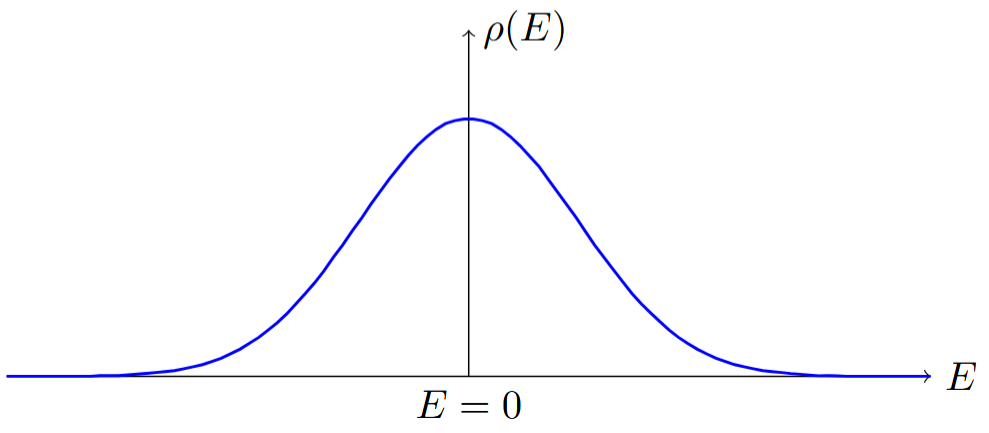
\includegraphics[width=.5\linewidth]{Figures/spectrum.png}
\caption{Energy spectrum of the DSSYK model in the limit $\lambda \rightarrow 0$. The energy are approximately gaussian distributed around $E_0$. \cite{Narovlansky:2023lfz}}
\label{fig:spectrum}
\end{figure}
If we keep the de Sitter static patch in mind it is reasonable to introduce the temperature $\beta_\text{dS}$, which in our SYK model is just an other variable. We can introduce it by time evolution with the imaginary time $\pm i \beta_\text{dS}/4$ of our operators. This gives us two different kinds of observables $\mathcal{O}^\pm$ connected by
\begin{equation}
    \mathcal{O}^-(\tau) = \mathcal{O}^+(\tau + \frac{i \beta_\text{dS}}{2} ).
\end{equation}
This leads to the definition of a 2x2 matrix of two-point functions
\begin{equation}
    G^{ab}_\Delta (\tau_2, \tau_1) = \bra{\Psi_\text{dS}} \mathcal{O}^a_\Delta (\tau_2) \mathcal{O}^b_\Delta (\tau_1) \ket{\Psi_\text{dS}},
\end{equation}
with $a, b = \pm$. As the different operators are connected by rotation on the thermal circle it is sufficient to calculate the Green's function 
\begin{equation}
    G^{++}_\Delta (\tau) = \int dE G^{++}_\Delta (E) e^{-i(E-E0)\tau}
\end{equation}
with $\tau = \tau_2 -\tau_1$. This boils down to the calculation of
\begin{equation}
    G^{++}_\Delta (E) = \rho(E) \, \left| \bra{E_0} \mathcal{O}^+_\Delta \ket{E} \right|^2
    \label{eq:Green_E}
\end{equation}
Because our operator factorizes and we explicitly know the spectral density and also the matrix elements $\bra{E_0}\mathcal{O}_\Delta \ket{E}$ are known for DSSYK we can simply compute the Green's function. The matrix element for our physical operator reads
\begin{align}
    \bra{E_0} \mathcal{O}^+_\Delta \ket{E} &= \bra{E_0} \mathcal{O}^L_{1-\Delta} \ket{E}_L \bra{E_0} \mathcal{O}^R_\Delta \ket{E}_R \\
    &= \sqrt{\frac{\Gamma_q(1- \Delta \pm i s_0 \pm i s)}{\Gamma_q(2 \Delta)}} \sqrt{\frac{\Gamma_q(\Delta \pm i s_0 \pm i s)}{\Gamma_q(2 - 2 \Delta)}}. \nonumber
\end{align}
This rather unhandy expression is simplified in the limit $\lambda \rightarrow 0$ and for the assumption that $|s_0 - s|$ is small, so $2s$ and $s + s_0$ scale like $1/\lambda$. 
In \cite{Narovlansky:2023lfz} it is described in detail how one can use the formula
\begin{equation}
    \Gamma_q(x) \Gamma_q(1-x) = \frac{i q^{1/8} (1-q) (q;q)^3}{q^{x/2} \, \vartheta_1(i \lambda x, q)}
\end{equation}
to simplify the matrix elements. If we plug in the explicit expressions for $\rho(E)$ and the matrix elements into \eqref{eq:Green_E} we get
\begin{equation}
    G^{++}_\Delta(E) = \rho_0 \, \vartheta_1(2 \lambda s, q) \, \frac{\vartheta_1(2 i \lambda \Delta, q)}{\vartheta_1(\lambda(i \Delta \pm s_0 \pm s), q)}.
\end{equation}
Here we take $s = s_0 - \omega /2$ to be in the proximity of $s_0 \gg \omega$, and we substitute $\Delta$ by $\mu = 1- 2\Delta$. If we finally take the limit $\lambda\rightarrow0$ and drop all the constant overall factors, the Green's function has the form
\begin{equation}
    G^{++}_\Delta (E)|_{\lambda = 0} = \frac{\sin{\pi \mu}}{\cosh{\frac{\pi}{2}(\omega + i \mu)} \cosh{\frac{\pi}{2}(\omega -i \mu) }}.
\end{equation}
By Fourier transforming this function, we get the self-correlation function analysed in numerically in the next part.

\section{Krylov complexity for the DSSYK model}
The goal of this section is to calculate the Krylov complexity for a pair of double-scaled SYK models coupled by an equal-energy constraint, as outlined in \cite{Narovlansky:2023lfz}. For this, we follow the procedure given in the appendix of \cite{Parker:2018yvk}. The starting point is the two-point function in the semi-classical limit obtained in the last section. In real space the Green's function reads
\begin{equation}
\label{2pf}
    G^{++}_\Delta(\tau)|_{\lambda=0}=\frac{2\sinh(\mu\tau)}{\pi \sinh{\tau}}.
\end{equation}
For simplicity, we will call this correlator $G(\tau)$ from now on.
\subsection{From moments to Lanczos coefficients}
The first step of the calculation consists of calculating the moments
\begin{equation}
    m_{2n}=(-1)^n\frac{d^{2n}}{dt^{2n}}G(t)|_{t=0}.
\end{equation}
For the correlator \eqref{2pf}, we find the following analytical expression for the moments:
\begin{equation}
    m_{2n}=\frac{2}{\pi}(-1)^n\frac{2^{2n+1}}{2n+1}B_{2n+1}\left(\frac{1+\mu}{2}\right).
\end{equation}
This result can be derived from the generating function of the Bernoulli polynomials $B_n(x)$:
\begin{equation}
    \label{genfct}
    \frac{ze^{xz}}{e^z-1}=\sum_{n=0}^{\infty}B_n(x)\frac{z^n}{n!},
\end{equation}
by using the redefinitions $z\rightarrow2t$ and $x\rightarrow\frac{1+\mu}{2}$. Then, we perform an antisymmetrization of equation \eqref{genfct}, i.e., we add the same equation with the replacement $t\rightarrow-t$. Thus, we obtain a series expansion for $G(t)$, from which the moments $m_{2n}$ can be read off directly.\\
The next step of our calculation is to determine the Lanczos coefficients, using the following recursion algorithm:
\begin{align}
    b_n &= \sqrt{M_{2n}^{(n)}},\\
    M_{2k}^{(m)} &= \frac{M_{2k}^{(m-1)}}{b^2_{m-1}}-\frac{M_{2k}^{(m-2)}}{b^2_{m-2}},\ k=m,...,n
\end{align}
We also use the following initial values: $b_{-1}=b_0=1$, $M_{2k}^{(-1)}=0$, and $M_{2k}^{(0)}=\mu_{2k}$. For the implementation of this algorithm, we use Mathematica.
\begin{figure}
    \centering
    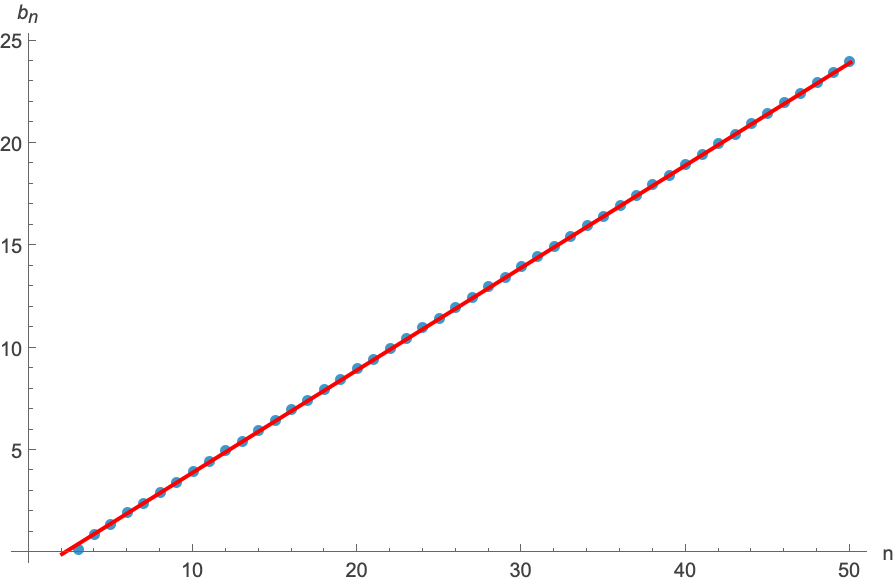
\includegraphics[width=0.5\linewidth]{Figures/lanczos_mu0.9.png}
    \caption{The first 50 Lanczos coefficients $b_n$ (blue) for $\mu=0.9$ with a linear fit (red)}
    \label{fig:lanczos}
\end{figure}
The results for the Lanczos coefficients $b$ are shown in Figure \ref{fig:lanczos}. The coefficients quickly asymptote to a linear function with a slope of $1/2$. Linear growth is in fact the maximal growth rate of Lanczos coefficients, and it is typical for a chaotic system like the SYK model \cite{Parker:2018yvk}. Another piece of evidence for linear Lanczos coefficients can be found by considering the spectral Green's function, which was given in \cite{Narovlansky:2023lfz} as the Fourier transform of \eqref{2pf}:
\begin{equation}
    G_\Delta(E)|_{\lambda=0}=\frac{\sin{\pi\mu}}{\cosh{\frac{\pi}{2}(\omega+i\mu)}\cosh{\frac{\pi}{2}(\omega-i\mu)}}=\frac{2\sin{\pi\mu}}{\cosh{\pi\omega}+\cos{\pi\mu}}
\end{equation}
From the second representation, which can be obtained by some simple manipulations, it is obvious that the spectral function decays exponentially ($\sim e^{-\pi\omega}$) for large $\omega$. In \cite{Parker:2018yvk}, it was shown that this corresponds to linearly growing Lanczos coefficients, giving a sanity check for our results.
\subsection{Numerical results for the complexity}
With the Lanczos coefficients calculated in the previous section, it is now straightforward to determine the time evolution of the Krylov complexity. In the Krylov basis, the Hamiltonian matrix $H$ is tridiagonal, with the main diagonal given by zeroes and the subdiagonal and supradiagonal given by the Lanczos coefficients. As an initial state, we take the lowest energy eigenstate $\ket{\psi_0}$ of $H$ and evolve it forwards in time by multiplying with $e^{iHt}$:
\begin{equation}
    \ket{\psi(t)}=e^{iHt}\ket{\psi_0}=\sum_{n\geq0}\psi_n(t)\ket{\psi_n}
\end{equation}
The Krylov complexity is then given by the expectation value of the number operator in the Krylov basis:
\begin{equation}
    C_K(t)=\sum_{n\geq0}n|\psi_n(t)|^2
\end{equation}
We perform the diagonalization and time evolution numerically in Python and obtain the results presented in Figure \ref{fig:kcomp}. We were able to run the calculation for up to 1000 Lanczos coefficients. For all numbers of Lanczos coefficients, the Krylov complexity increases exponentially at early times $t\lesssim7$. This behavior is typical for chaotic systems with linearly increasing Lanczos coefficients \cite{Parker:2018yvk}. However, at later times, the complexity reaches a peak and then decreases again. We believe this to be a numerical artifact, since the peak is shifted to later times when more Lanczos coefficients are included. If we were able to calculate an arbitrary number of Lanczos coefficients, then the Krylov complexity would continue to increase indefinitely. 
\begin{figure}[h!]
    \centering
    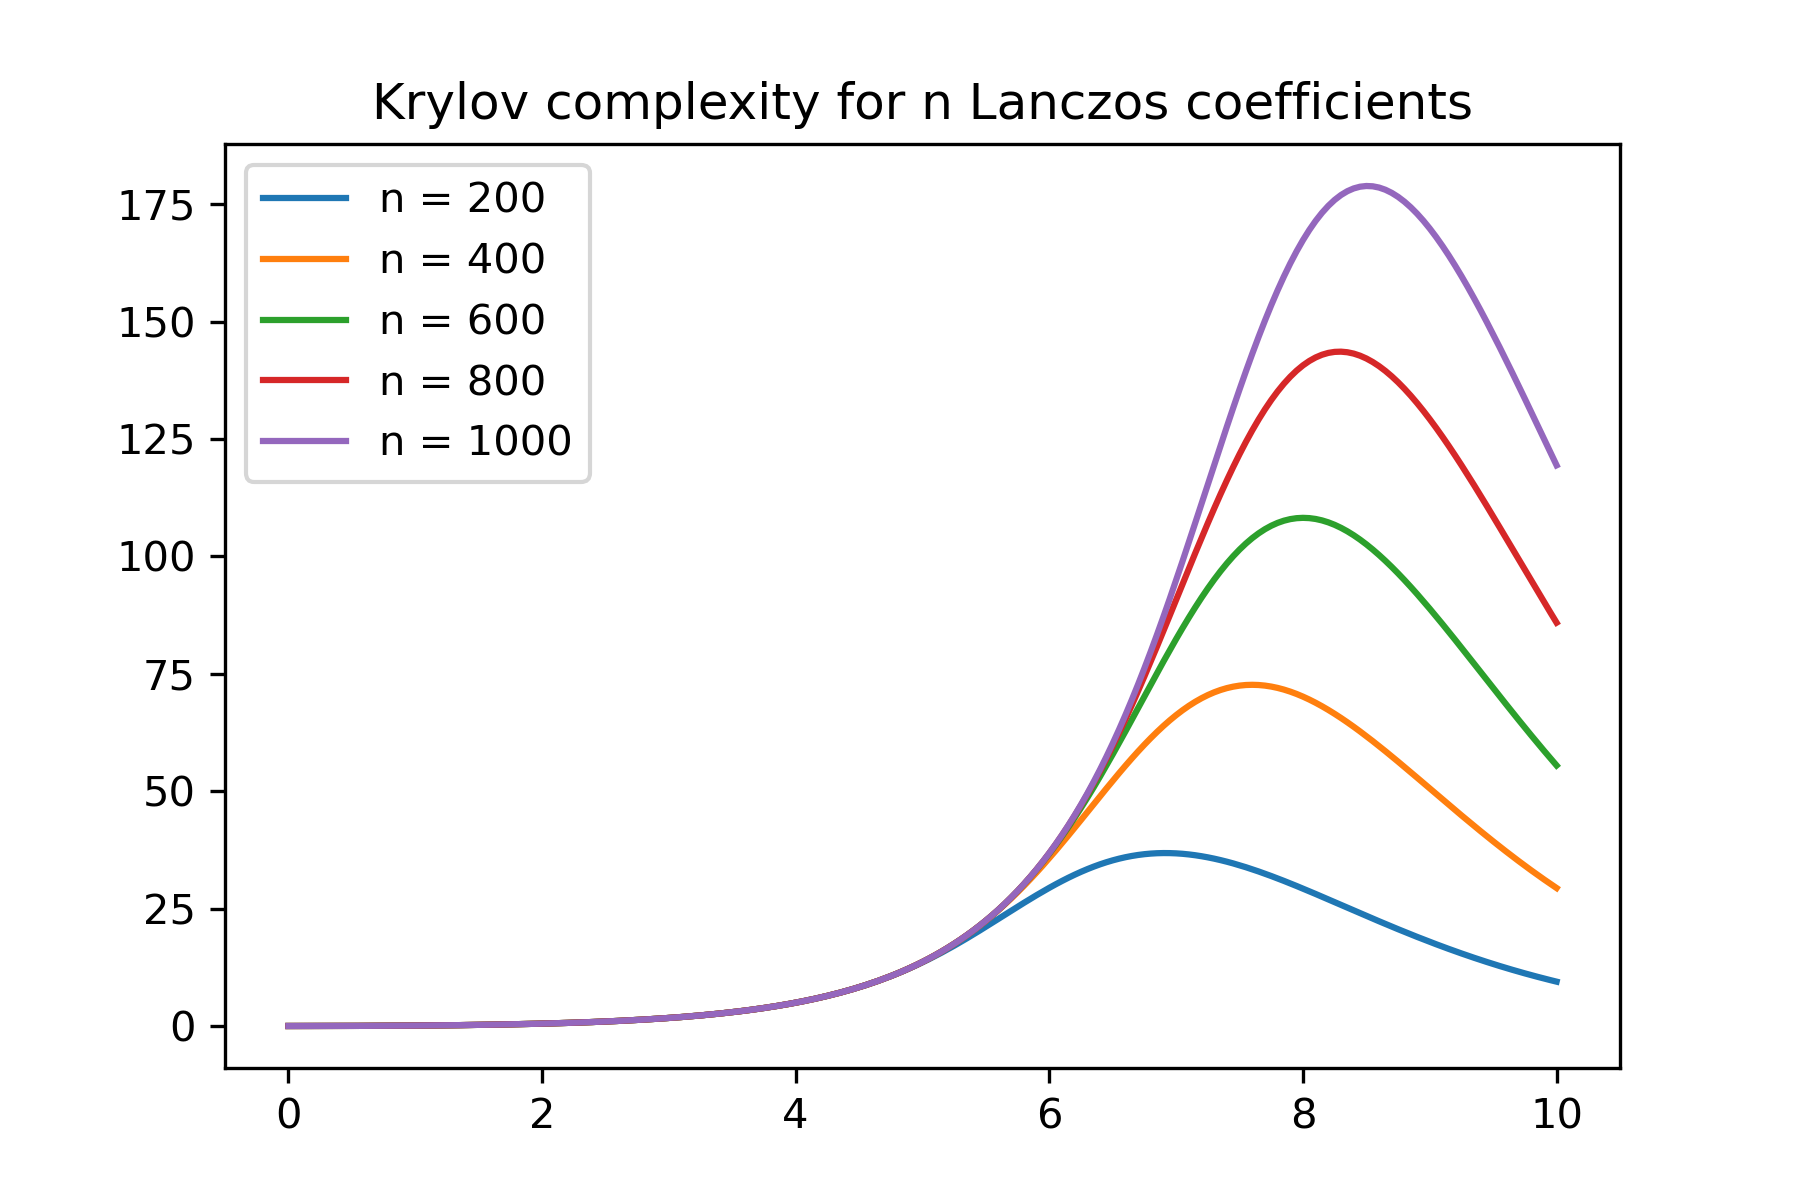
\includegraphics[width=0.6\linewidth]{Figures/dssyk_kcomplexity.png}
    \caption{We plot the time evolution of the Krylov complexity for different numbers of Lanczos coefficients.}
    \label{fig:kcomp}
\end{figure}

\subsection{Spectral form factor}

As a second characteristic measure for quantum chaos, we can look at the spectral form factor (SFF). As in \cite{erdmenger_universal_2023} we can write the SFF as 
\begin{equation}
    \left|Z(\beta + i t) \right|^2 = \left|\text{Tr} \, e^{-(\beta + i t )H}\right|^2
\end{equation}
We calculate the SFF for real times $t$ with the Krylov space Hamiltonian
\begin{equation}
    H_\text{Krylov} = 
    \begin{pmatrix}
    0 & b_1 & 0  & \cdots \\
    b_1 & 0 & b_2 &  \\
    0 & b_2 & 0 & \ddots \\
    \vdots & & \ddots & \ddots
    \end{pmatrix},
\end{equation}
which gives us 
\begin{equation}
    \text{SFF}(t) = \left| \sum_n e^{-i E_n t}\right|^2.
\end{equation}
For different values of $n$ we calculated and compared the SFF (fig. \ref{fig:sff}). Also here we can see some numerical artifacts as e.g. the oscillation period increases with increasing $n$.
\begin{figure}[htbp]
    \centering
    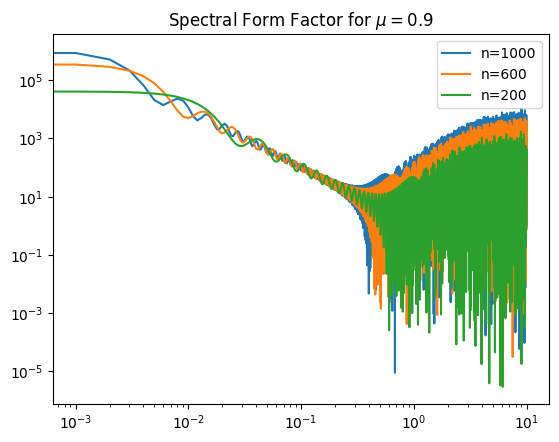
\includegraphics[width=0.6\linewidth]{Figures/sff__09.png}
    \caption{Spectral form factor for different number $n$ of Lanczos coefficients with $\mu  = 0.9$}
    \label{fig:sff}
\end{figure}
\newpage
\printbibliography
\end{document}
